The concept of Human-AI Teaming for cybersecurity is motivated by limitations on both sides of the human–machine spectrum. Cyber agents excel in high-frequency detection, large-scale log processing, and consistent execution of defensive playbooks, making them invaluable during rapidly unfolding attacks such as lateral movement, credential escalation, or large-scale scanning. However, these agents lack contextual awareness, cannot interpret multi-domain implications (e.g., mission importance of an OT asset), and may recommend actions that inadvertently disrupt operations.
In contrast, human defenders possess strong contextual understanding, creativity, intuition, and ethical judgment, especially important during complex or novel attacks. Yet they struggle with the speed and volume of modern cyber engagements and can become overloaded or inconsistent under stress.

For example, let's say a Blue agent detects a privilege escalation on a subnet supporting admin systems and safety controllers. 
It decides to isolate the segment as there is a  92\% mitigation chance and only a 35\% risk of alerting the attacker. 
However, what the agent doesn't consider is that full isolation would raise operational risk during a maintenance cycle. 
So, with this contextual knowledge the human narrows the response to a subset of hosts and applies rapid policy updates, preserving mission continuity while mitigating the threat. 
The agent executes, monitors, and logs the action, showing that collaboration, not full autonomy, is essential.

To allow for this collaboration, we develop a system where human operators can override AI teammates and inject alternative actions whenever they disagree on attack or defense trajectories. 
To support issue detection and diagnosis, we provide two forms of explanations-direct and counterfactual-for agent actions, accessible through an LLM-based chatbot for ease of use. 
Finally, we integrate these explanations into a unified dashboard, where each action is annotated with its probability of success, expected execution time, likelihood of attacker detection, and impact on overall risk profile of the network \cite{neema2021model}.
A control loop in our developed system is shown in Figure \ref{fig:human_ai_loop}.

\begin{figure}[t]
\centering
\resizebox{\columnwidth}{!}{
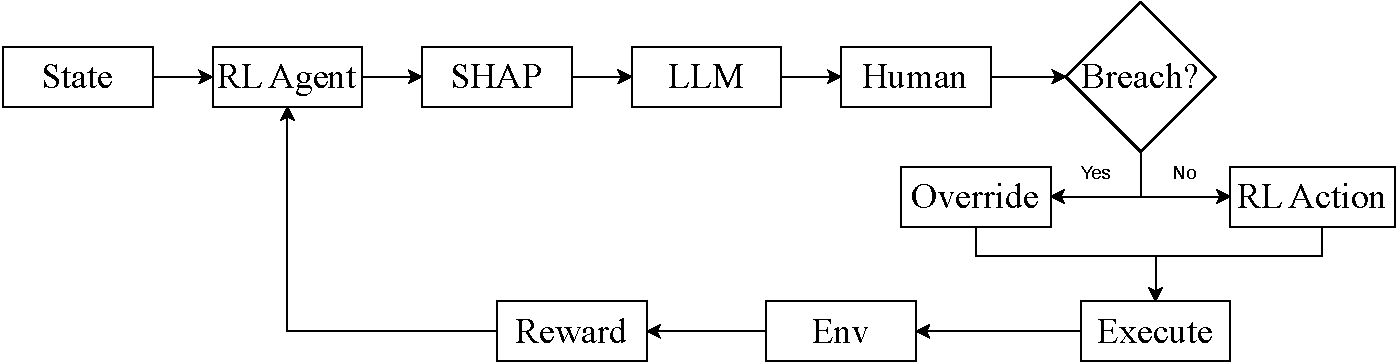
\includegraphics[]{Figures/flow_DESTION.drawio.pdf}
}
\caption{Human--AI cyber defense control loop with intervention condition.}
\label{fig:human_ai_loop}
\end{figure}